A continuación, se describen los métodos de mitigación a nivel de algoritmo estudiados: la Loss Focal, el PRM-IM, la red sensible a costes (CoSenCNN), y la novedosa Loss Focal Difusa. %Además, y como novedad de este trabajo, se ha modificado la Loss Focal con inspiración en otros trabajos (\cite{patel2017classification,cho2020instance,liu2017fuzzy}), para tratar de mejorar su rendimiento. Se ha llamado a este método la Loss Focal Difusa. (subrayados en la Tabla \ref{TB:ALGO_DISCARD})

%%%%%%%%%%%%%%%%%%%%%%%%%%%%%%%%%%%%%%%%%%%%%%%%%%%%
\subsection{Loss Focal\label{SUBSEC:FOCAL_LOSS}}
%%%%%%%%%%%%%%%%%%%%%%%%%%%%%%%%%%%%%%%%%%%%%%%%%%%%

La Entropía Cruzada (en adelante, \textit{Cross Entropy} ó CE), es una función de pérdida que funciona bien en muchos escenarios, pero ve su efectividad reducida cuando las clases están desbalanceadas \cite{hong2021fuzzy}. En \citet{lin2017focal} proponen la llamada \textit{Loss Focal}, que centra su aprendizaje en las muestras minoritarias, como sustituto de la pérdida por entropía cruzada. Aplicándola al desbalanceo en problemas de detección de objetos, los autores encontraron una mejora sustancial en todas las métricas recogidas cuando se comparaban a otras del estado del arte \cite{lin2017focal}. Matemáticamente:

\begin{equation}[EQ:FOCAL_LOSS]{Fórmula de la \textit{Focal Loss}.}
   Focal\ Loss = -\sum_{n=1}^{m}{T_n log\ t_n (1 - t_n)^\gamma}
\end{equation}

Donde $m$ el número de clases, $T_n$ es la clase real de la muestra y $t_n$ es probabilidad o ``confianza'' para la clase predicha. El factor $(1 - t_n)^\gamma$ es el encargado de modular el valor de la función de pérdida: cuando $t_n$ es pequeña, el factor es muy cercano a 1 y por tanto la pérdida no cambia. A medida que $t_n \rightarrow 1$, el factor se acerca a 0 y la pérdida para muestras bien clasificadas se degrada. Intuitivamente, este ``factor modulador'' reduce la contribución de las muestras ``fáciles'' (alta $t_n$), y extiende el rango en que una muestra recibe una pérdida baja. Cabe resaltar cómo, sin este factor (o si $\gamma = 0$), la Loss Focal no es más que la pérdida por Entropía Cruzada. La Figura \ref{FIG:FOCAL_LOSS_CURVE} resume las características de esta función de pérdida.

\begin{figure}[Curva de la Loss Focal]{FIG:FOCAL_LOSS_CURVE}{Curvas de pérdida para la Loss Focal bajo diversos valores de $\gamma$.}
    \image{10cm}{}{focal_loss_curve}
\end{figure}

%%%%%%%%%%%%%%%%%%%%%%%%%%%%%%%%%%%%%%%%%%%%%%%%%%%%
\subsection{PRM-IM\label{SUBSEC:PRMIM}}
%%%%%%%%%%%%%%%%%%%%%%%%%%%%%%%%%%%%%%%%%%%%%%%%%%%%

En \citet{rahimzadeh2020modified}, se ataca el problema de desbalanceo en un dataset de radiografías con covid-19 por medio de una estructura que combina dos extractores de características basados en CNNs, y un algoritmo de repetición que permite al modelo revisar la clase minoritaria más veces que la mayoritaria. La técnica original surge de \citet{ghanem2008learning}, donde se aplica a procesamiento del lenguaje y recibe el nombre de PRM-IM (del inglés \textit{Probabilistic Relational Model for IMbalanced class problem}). El modelo propuesto en \citet{rahimzadeh2020modified} adapta la idea anterior al problema del desbalanceo en clasificación de radiografías de pulmones infectados con covid-19 y neumonía, mejorando las métricas para la clase más infrarrepresentada (covid-19) con una Accuracy del 90\%. La Figura \ref{FIG:PRM-IM} muestra el flujo de dicho sistema, ejemplificado para nuestro dominio de la clasificación de género.

\begin{figure}[Esquema de un PRM-IM]{FIG:PRM-IM}{Esquema de flujo en el sistema PRM-IM de \cite{rahimzadeh2020modified}.}
    \image{13cm}{}{prm-im}
\end{figure}

Los datos se dividen entre entrenamiento y validación, en un ratio 70-30\%. Para el subconjunto de entrenamiento, sean $M$ y $m$ los tamaños de la clase mayoritaria y minoritaria, respectivamente. A partir de ahí:

\begin{enumerate}
    \fontsize{11pt}{12pt}\selectfont
    \item Se dividen los datos de entrenamiento en $k = \frac{M}{m}$ subconjuntos. Cada uno estará formado por las $m$ muestras de la clase minoritaria, y un subconjunto único de $m$ muestras de la clase mayoritaria $M_i, i \in \{1, ..., k\}$.
    \item Durante $E$ épocas de entrenamiento, iterar sobre los $k$ subconjuntos:
    \begin{enumerate}
        \fontsize{11pt}{12pt}\selectfont
        \item Para cada muestra de los $k$ subconjuntos:
        \begin{enumerate}
            \fontsize{11pt}{12pt}\selectfont
            \item Se introduce la muestra en dos extractores convolucionales en paralelo: uno se basa en \textit{Xception} \cite{chollet2017xception}, y el otro en \textit{ResNet50} \cite{he2016deep}, ambas sin la parte densamente conexa (sólo las capas convolucionales).
            \item Los vectores de características resultantes se concatenan y se hacen pasar por una última capa convolucional, aplanando su salida.
            \item Este vector aplanado se hace pasar por un clasificador formado por capas densamente conexas, para producir finalmente una predicción para cada una de las clases del problema (previa activación por Softmax).
        \end{enumerate}
    \end{enumerate}
\end{enumerate}

Así, el propósito de la arquitectura es, en esencia, que el modelo sea expuesto a la clase minoritaria más veces que a la mayoritaria, para compensar por el desbalanceo presente, y dependiendo el ``número de exposiciones'' en el grado de desbalanceo ($k = \frac{M}{m}$). Todo ello, sin alterar la distribución de clases del conjunto de datos (es decir, sin aplicar sobremuestreo en ningún momento).

Otras investigaciones han sugerido métodos de \textit{ensemble} basados en esta idea, como \citet{guo2004learning}. No obstante, en este proyecto se implementa la arquitectura de la Figura \ref{FIG:PRM-IM} para las comparaciones por sus resultados prometedores (más de 93\% de F1-score en el campo de las radiografías de covid-19 y neumonía).

%%%%%%%%%%%%%%%%%%%%%%%%%%%%%%%%%%%%%%%%%%%%%%%%%%%%
\subsection{Red sensible a costes (CoSenCNN)\label{SUBSEC:COSEN_NET}}
%%%%%%%%%%%%%%%%%%%%%%%%%%%%%%%%%%%%%%%%%%%%%%%%%%%%

En \citet{khan2017cost}, se reduce el sesgo hacia la clase mayoritaria utilizando el concepto de aprendizaje con costes. En este escenario, la función de costes penaliza al clasificador por las clasificaciones erróneas de distinta forma dependiendo de qué clase se está clasificando mal. En concreto, una matriz de costes define que la penalización por clasificar una muestra minoritaria como mayoritaria es mayor que si se clasifica una muestra mayoritaria como minoritaria.

La matriz de costes es una estructura $\mathcal{E}_{p,q}$ donde $\mathcal{E}_{p,p} = 0\,\forall p$ y $\mathcal{E}_{p,q} > 0\,\forall p,q$. Su función es tomar las salidas de la red convolucional que conforma el modelo y aplicar los costes antes de pasar por la función de pérdida (es decir, se aplica sobre los llamados \textit{logits}). La función de pérdida en este caso es la de entropía cruzada. Los autores definen, pues, el siguiente modelo de funcionamiento del clasificador (Figura \ref{FIG:COSEN_NET}):

\begin{figure}[Esquema de la red sensible a costes (CoSenCNN)]{FIG:COSEN_NET}{Esquema de funcionamiento en la red sensible a costes (CoSenCNN). Imagen de: \citet{khan2017cost}.}
    \image{9cm}{}{CoSenNet}
\end{figure}

Los valores de la matriz de coste, $\mathcal{E}_{p,q}, p \neq q$, se aprenden junto a los pesos de la red convolucional durante el proceso de entrenamiento.

%%%%%%%%%%%%%%%%%%%%%%%%%%%%%%%%%%%%%%%%%%%%%%%%%%%%
\subsection{Loss Focal Difusa\label{SUBSEC:FUZZY_LOSS}}
%%%%%%%%%%%%%%%%%%%%%%%%%%%%%%%%%%%%%%%%%%%%%%%%%%%%

La motivación de querer diseñar un método algorítmico frente a uno a nivel de datos es que se ha demostrado que los primeros tienen menor probabilidad de afectar a los tiempos de entrenamiento. En esencia, suelen ser más fáciles de ``portar'' a diferentes problemas con un tuneado de parámetros mínimo. Es por ello que se considera que debe hacerse un esfuerzo por desarrollar métodos más eficientes dentro de esta familia.

La Loss Focal (Sección \ref{SUBSEC:FOCAL_LOSS}) tiene el inconveniente de que el parámetro $\gamma$ mantiene un mismo valor para todas las clases, y durante todo el proceso de entrenamiento. En \citet{hong2021fuzzy}, se propone que a mayor tamaño de clase (mayor \textit{grado de balanceo} respecto a dicha clase), mayor sea el valor de $\gamma$, pero los autores de este artículo siguen manteniendo el mismo valor durante todo el aprendizaje. Como el objetivo es minimizar la función de pérdida, la idea intuitiva es que a mayor $\gamma$, menor sea la Loss (Ecuación \ref{EQ:FOCAL_LOSS}); y a menor $\gamma$, mayor Loss. Con esto se pretende que las muestras pertenecientes a la clase mayoritaria tengan una menor pérdida, facilitando su aprendizaje; mientras que las muestras de la clase minoritaria tendrán una mayor pérdida, y se les deberá prestar más atención para aprenderlas.

Por otra parte, durante el estudio bibliográfico se ha dado con varios estudios \cite{patel2017classification,cho2020instance,liu2017fuzzy} en los que se hace uso de lógica difusa en algoritmos de aprendizaje automático. Vemos en \citet{burduk2008possibility} cómo se diseña una función de pérdida basada en reglas linguísticas difusas; en \citet{cho2020instance} cómo se modifica un SVM difuso (FSVM) para compensar el desbalanceo; o en \citet{patel2017classification} como hacen lo propio con un algoritmo de vecinos próximos. Es por ello que se plantea en este trabajo la idea de aplicar lógica difusa para mejorar las deficiencias detectadas en la Loss Focal tradicional, y dar lugar a un método llamado Loss Focal Difusa. Para dar un poco de contexto, un Sistema de Control Difuso (FCS) de Mamdani \cite{mamdani1974application} tiene tres componentes, que ilustra la Figura \ref{FIG:FCS_EXPLAINED}:

\begin{figure}[Esquema de un FCS]{FIG:FCS_EXPLAINED}{Esquema de flujo de información de un sistema de control difuso (FCS).}
    \image{10cm}{}{fcs_explained}
\end{figure}

\begin{enumerate}
    \fontsize{11pt}{12pt}\selectfont
    \item El \textit{fuzzifier} convierte la entrada a variables linguísticas de acuerdo a funciones de pertenencia (``\textit{membership functions}'') predefinidas.
    \item Una base de reglas linguísticas es usada para inferir conclusiones en base a las variables de entrada.
    \item El \textit{defuzzifier} convierte las conclusiones a variables del mismo formato que la entrada.
\end{enumerate}

Para definir la base de reglas y funciones de pertenencia del FCS de la Loss Focal Difusa, se ha pensado en la forma en que deben variar las pérdidas de ambas clases, mayoritaria y minoritaria, y en el papel del parámetro $\gamma$ en todo ello. Se sabe que cuanto mayor es una clase, menor debe ser su pérdida (y viceversa), y también se quiere que ésta se modifique de forma activa durante el aprendizaje por medio de modificar el valor del parámetro $\gamma$ para cada clase, para compensar las muestras difíciles de aprender. Entonces surge la duda de cuán grande debe ser esa variación de $\gamma$, y si esta debe ser positiva (aumentar) o negativa (disminuir). Así, de forma similiar a como \citet{patel2017classification} modifican el algoritmo de K-vecinos ponderado para modificar de forma difusa los pesos, aquí se utiliza un FCS para modificar el valor del parámetro $\gamma$ para cada clase, al acabar cada iteración del aprendizaje. Dicho FCS tiene dos entradas. La primera es el grado de balanceo de cada clase (la inversa del IR de la Ecuación \ref{EQ:IMBRAT}):

\begin{equation}[EQ:BALANCE_DEG]{Fórmula del grado de balanceo para una clase i.}
   GB^i = \frac{tama\tilde{n}o\ clase_i}{Max(tama\tilde{n}o\ clase_i)} \leq 1, \;\; i \in {0,1} \;\; \text{para clasificación binaria.}
\end{equation}

La segunda entrada es el valor de la Loss para cada clase en la iteración anterior, $L^i_{t-1}$, y su propósito es acoplar el aprendizaje pasado a la actualización de $\gamma$ en la iteración presente (idea inspirada por \citet{burduk2008possibility}). Tanto $GB^i$ como $L^i_{t-1}$ pueden tomar los valores ``alto'', ``medio'' y ``bajo''. Por otra parte, la salida del FCS es la variación del parámetro $\gamma$, que puede ser ``positivo'' (aumenta), ``negativo'' (disminuye) o ``cero''. Las funciones de pertenencia para las entradas y la salida se han diseñado como triangulares por ser rápidas de computar, y se ilustran en la Figura \ref{FIG:FCS_INPUT_OUTPUT}. El dominio de la función de pertenencia para la variable $L^i_{t-1}$ se ha determinado empíricamente por la variación máxima de la pérdida en la Loss Focal tradicional. Por su parte, el dominio de $GB^i$ solo puede variar, por definición, entre 0 y 1. Los límites de la salida se establecen entre -0,2 y 0,2 para evitar que la variación de $\gamma$ sea muy abrupta de una iteración a otra.

\begin{figure}[Funciones de pertenencia del FCS]{FIG:FCS_INPUT_OUTPUT}{Funciones de pertenencia para las entradas (arriba) y la salida (abajo) del sistema de control de la Loss Focal Difusa.}
    \centering
    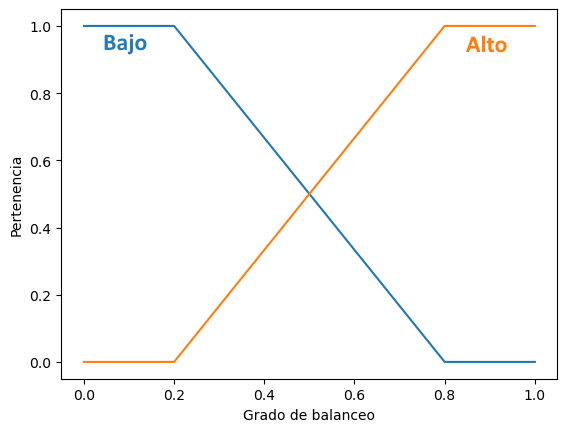
\includegraphics[width=7cm]{img/fcs_input_1.png}
    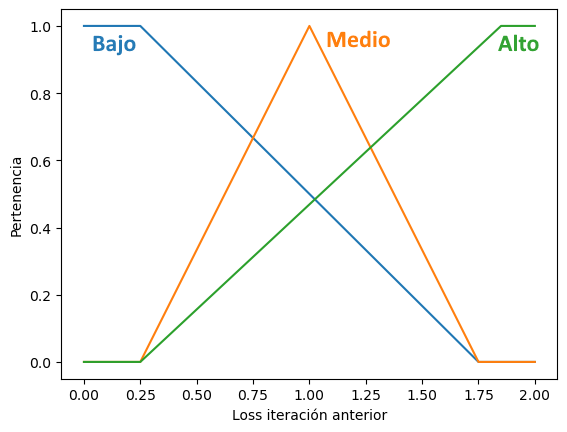
\includegraphics[width=7cm]{img/fcs_input_2.png}
    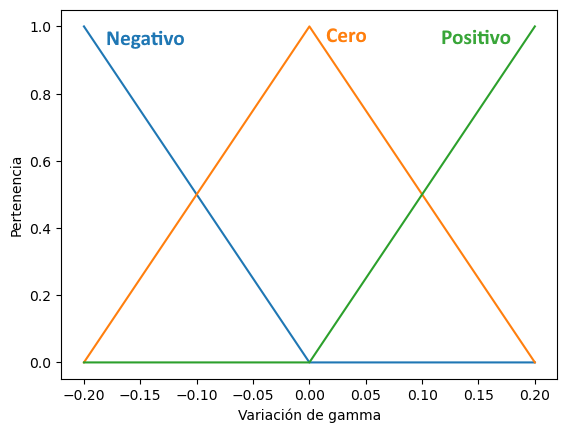
\includegraphics[width=7cm]{img/fcs_output.png}
\end{figure}

Por último, y de acuerdo a las relaciones entre la actualización de $\gamma$ y el tamaño de clases que ya se han razonado, se propone la siguiente base de reglas:

\begin{enumerate}
    % \fontsize{11pt}{11pt}\selectfont
    \item \textbf{Regla 1}: SI $GB^i$ ES ``bajo'' Y $L^i_{t-1}$ ES ``bajo'' ENTONCES delta\_gamma ES ``\textit{negativo}''
    \item \textbf{Regla 2}: SI $GB^i$ ES ``bajo'' Y $L^i_{t-1}$ ES ``medio'' ENTONCES delta\_gamma ES ``\textit{negativo}''
    \item \textbf{Regla 3}: SI $GB^i$ ES ``bajo'' Y $L^i_{t-1}$ ES ``alto'' ENTONCES delta\_gamma ES ``\textit{cero}''
    \item \textbf{Regla 4}: SI $GB^i$ ES ``alto'' Y $L^i_{t-1}$ ES ``bajo'' ENTONCES delta\_gamma ES ``\textit{cero}''
    \item \textbf{Regla 5}: SI $GB^i$ ES ``alto'' Y $L^i_{t-1}$ ES ``medio'' ENTONCES delta\_gamma ES ``\textit{positivo}''
    \item \textbf{Regla 6}: SI $GB^i$ ES ``alto'' Y $L^i_{t-1}$ ES ``bajo'' ENTONCES delta\_gamma ES ``\textit{positivo}''
\end{enumerate}

Con estas reglas, se logra una Loss elevada para la clase minoritaria (bajo $GB^i$), y una Loss reducida para la mayoritaria (alto $GB^i$), pero la actualización dinámica de $\gamma$ pretende además ``sortear'' las muestras difíciles que aparezcan durante el entrenamiento. Finalmente, para convertir las salidas de las reglas a un valor de actualización de $\gamma$, se usa el método de centroides para ``\textit{deffuzificar}'', pues es el estándar en la bibliografía especializada \cite{patel2017classification,cho2020instance,liu2017fuzzy,Kiefner_FuzzyLogic_for_Python_2022}.

% Cabe mencionar que la introducción de la Loss Focal Difusa no añade prácticamente ninguna diferencia al entrenamiento con la Loss Focal clásica, más allá de incluir la actualización del parámetro $\gamma$, por medio del FCS diseñado, al finalizar cada iteración del aprendizaje.

% \begin{equation}[EQ:MAMDANI_CENTROID]{Fórmula del método de centroides de Mamdani.}
%     \gamma = \frac{\sum_{k=1}^N{a_k \times \overline{x_k}}}{\sum_{k=1}^N{a_k}}
% \end{equation}

% Donde $N$ indica el número de sub-áreas, y $a_k$ y $\overline{x_k}$ son el área y el centroide del sub-área k-ésima, respectivamente.